% !TeX root = ../main.tex
% !Mode:: "TeX:UTF-8"
\section{第七章 风险分析}\label{ux7b2cux4e03ux7ae0-ux98ceux9669ux5206ux6790}

PI OS 面向企业智能体的高密度部署需求，通过运行时扁平化、动态资源卸载和智能内存共享，提高有限服务器资源的利用效率。项目已完成现阶段核心代码开发，后续将围绕命题环境适配、产品交付和商业转化推进。随着项目从研究验证走向企业应用，需要重点管理市场接受度、运行可靠性、资金投入和成果使用等风险。

\subsection{7.1 风险识别}\label{ux98ceux9669ux8bc6ux522b}

\subsubsection{7.1.1 市场风险}\label{ux5e02ux573aux98ceux9669}

\NumberedPara{1}{技术收益与客户采购需求存在差异}

PI OS 的商业价值在于帮助客户利用相同设备承载更多智能体任务，降低部署和运行成本。但不同客户的业务结构存在差异：部分任务等待时间较短，可回收的资源有限；部分客户的主要开支来自模型调用，沙箱资源所能节省的占比有限，对整体成本的改善不明显。因此，实验中的性能提升需要结合客户实际业务，才能判断是否具有采购价值。

\NumberedPara{2}{客户验证周期较长}

企业引入基础软件通常需要经过兼容性测试、安全审查、试运行和采购审批。即使客户认可技术方案，也可能因现有系统改造成本、预算安排和运维习惯而推迟采购，影响项目收入形成的速度。

\NumberedPara{3}{竞争与客户集中风险}

云平台、智能体开发平台和沙箱服务商可能通过价格调整、产品升级或捆绑服务参与竞争。若项目早期对单一合作方依赖过高，其需求调整或采购延期，可能使项目在短期内出现收入缺口。

\begin{center}
\begin{minipage}{\linewidth}
\centering
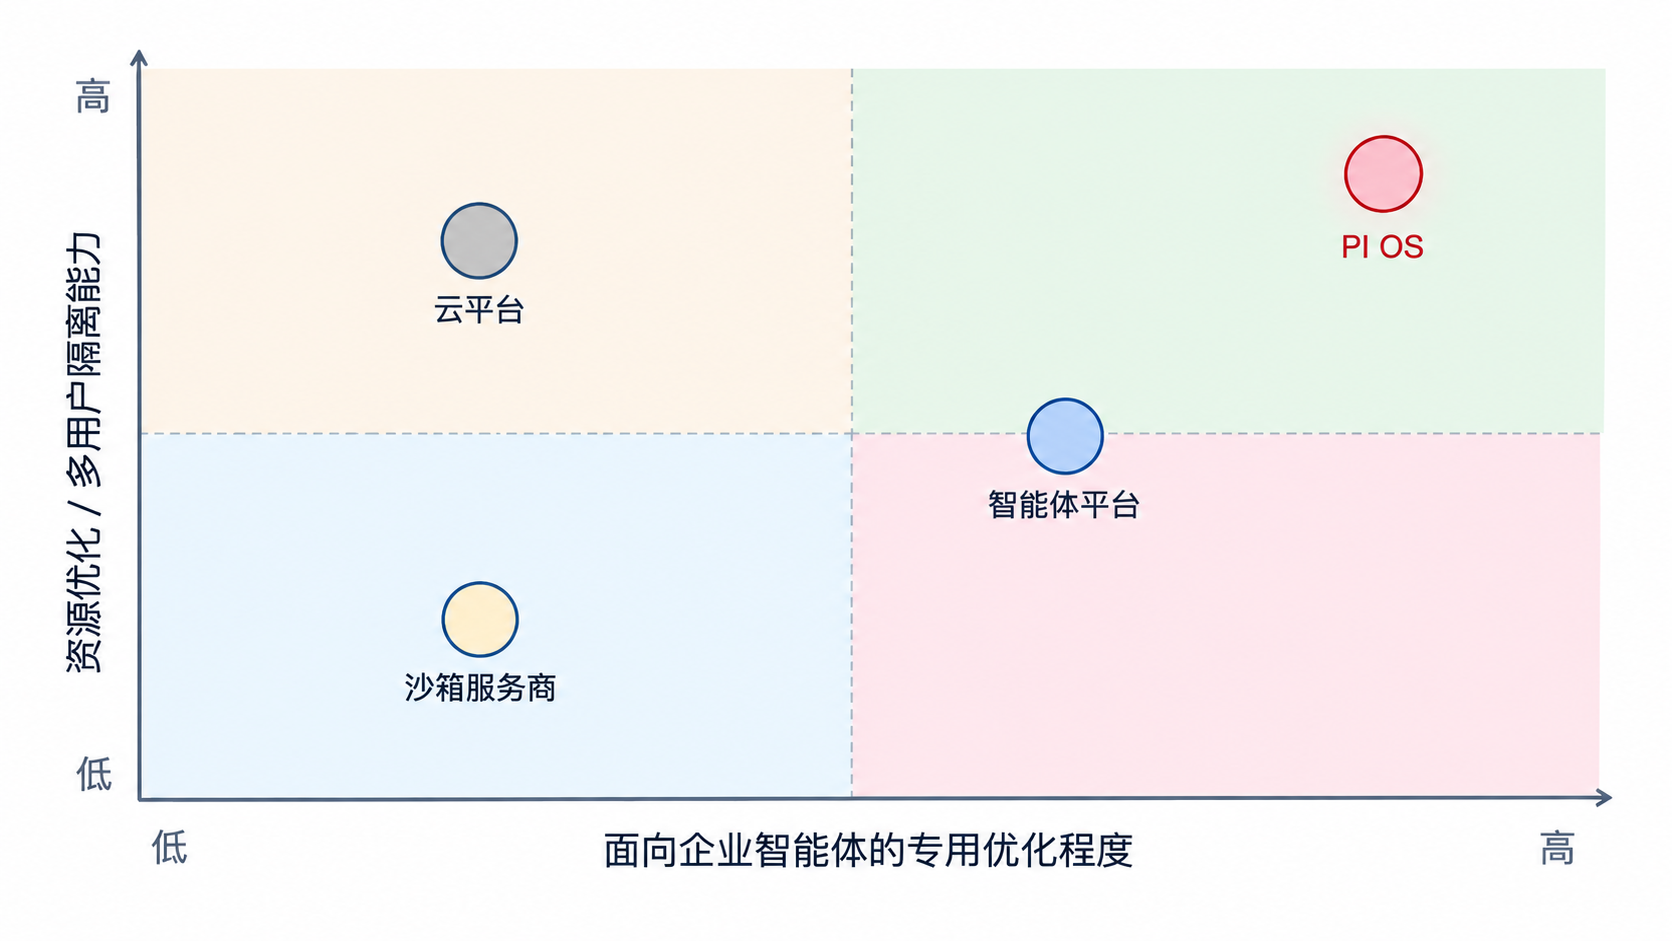
\includegraphics[width=5.5in,keepaspectratio]{figures/image24.png}
\WordFigureCaption{图 7-1 PI OS 与主要竞争方案的定位对比}
\end{minipage}
\end{center}

\subsubsection{7.1.2 操作风险}\label{ux64cdux4f5cux98ceux9669}

\NumberedPara{1}{资源优化影响任务连续性}

动态资源卸载需要在适当时机保存任务状态，并在任务继续执行时准确恢复。若状态保存不完整、恢复顺序错误或异常处理不足，可能导致任务中断、结果错误或外部操作重复执行，进而影响客户业务连续性。

\NumberedPara{2}{高密度部署放大资源波动}

多个智能体同时恢复运行时，可能集中申请内存和读取存储，形成瞬时资源高峰。若调度策略不当，单个任务的异常可能波及同批其他任务，降低整体服务稳定性。

\NumberedPara{3}{研发与交付衔接不足}

核心代码完成后，仍需完善安装部署、监控告警、升级回退和故障处理等工程能力。若过早扩大交付范围，可能出现技术人员长期投入客户现场、维护成本增加和版本管理混乱等问题。

\subsubsection{7.1.3 财务风险}\label{ux8d22ux52a1ux98ceux9669}

\NumberedPara{1}{研发投入与收入形成存在时间差}

项目需要持续投入人员、测试设备、基础软件适配和客户验证，而商业收入取决于合同签订、交付进度与客户验收。当资金集中投入而收入回款滞后于交付进度时，可能出现阶段性现金流缺口。

\NumberedPara{2}{定制开发侵蚀项目利润}

不同客户的操作系统、业务工具和部署要求存在差异。若报价未充分考虑适配、维护和售后成本，即使取得订单，也可能因交付投入过高而难以形成合理利润。

\NumberedPara{3}{可用资金判断失准}

科研合作经费、创业投入和经营收入具有不同的使用范围与核算要求。合同约定金额也可能分阶段支付，若将合同约定金额全部视为可立即动用的经营资金，可能因提前投入而导致预算超支。

\subsubsection{7.1.4 法律风险}\label{ux6cd5ux5f8bux98ceux9669}

\NumberedPara{1}{科研成果商业化权属风险}

PI OS 的研究基础涉及校企合作，相关代码、技术文档和新增成果的使用，需要结合合作协议确认权属及授权范围。如果商业化主体、许可方式和收益安排未明确，可能影响产品销售、融资和后续合作。

\NumberedPara{2}{开源软件与第三方依赖风险}

项目使用的操作系统、虚拟化组件和工具包可能适用不同的开源许可证（如 GPL、Apache 2.0、MIT、MPL 等）。若未能识别相关许可证义务，可能影响代码分发、产品交付，甚至带来客户合规使用风险。

\NumberedPara{3}{合作信息披露风险}

企业合作信息、合同内容及研发资料可能受到保密约定限制。宣传材料、赛事展示和融资沟通若超出允许披露的范围，可能影响合作关系及项目信誉。

\subsubsection{7.1.5 数据与隐私风险}\label{ux6570ux636eux4e0eux9690ux79c1ux98ceux9669}

\NumberedPara{1}{跨客户数据边界不清}

不同客户访问权限划分不清，或共享范围、日志记录和任务清理机制不完善，可能出现跨任务数据泄露、凭据误用和敏感信息残留。

\NumberedPara{2}{敏感信息留存风险}

资源卸载形成的状态文件、运行日志及共享内存对象可能包含客户源代码、业务文件、访问凭据等信息，留存不当会直接损害客户信任。

\subsubsection{7.1.6 环境风险}\label{ux73afux5883ux98ceux9669}

\NumberedPara{1}{部署环境变化影响运行效果}

处理器架构、操作系统版本、存储性能和业务任务差异，都可能影响 PI OS 的资源节省与任务恢复效果。研究环境中的结果不能直接代表所有企业环境中的表现，命题指定环境与客户实际环境均需分别验证。

\NumberedPara{2}{客户预算和行业需求变化}

企业信息化预算调整、智能体应用落地节奏变化以及采购政策调整，可能改变客户的投资优先级。如果产品开发和市场拓展节奏与实际需求脱节，可能增加资金和人员投入压力。

\subsubsection{7.1.7 供应链风险}\label{ux4f9bux5e94ux94feux98ceux9669}

\NumberedPara{1}{上游更新与接口调整}

操作系统、虚拟化组件、语言环境、工具包和外部模型服务的版本更新、接口调整、服务中断或支持策略变化，会增加适配成本，影响复现与交付。

\NumberedPara{2}{单点依赖}

若对单一软件组件或服务商依赖较强，其停止维护、调整价格或发生故障时，项目可能缺乏替代方案。

\subsubsection{7.1.8 风险评估矩阵}\label{ux98ceux9669ux8bc4ux4f30ux77e9ux9635}

采用``发生概率（高/中/低）× 影响程度（高/中/低）''两个维度，对 7.1.1--7.1.7 识别的各类风险进行定级，并据此确定管理优先级。优先级参考以下规则：

高：概率与影响至少一项为``高''，且另一项不低于``中''

\begin{quote}
高风险类需重点管理、持续监测；
\end{quote}

中：概率与影响均为中，或一项高但另一项低

\begin{quote}
中风险类纳入常规管理；
\end{quote}

低：概率与影响均为低

\begin{quote}
低风险类可接受，按需关注。
\end{quote}

\begin{longtable}[]{@{}
  >{\centering\arraybackslash}p{(\linewidth - 10\tabcolsep) * \real{0.1080}}
  >{\centering\arraybackslash}p{(\linewidth - 10\tabcolsep) * \real{0.0679}}
  >{\centering\arraybackslash}p{(\linewidth - 10\tabcolsep) * \real{0.0679}}
  >{\centering\arraybackslash}p{(\linewidth - 10\tabcolsep) * \real{0.0740}}
  >{\raggedright\arraybackslash}p{(\linewidth - 10\tabcolsep) * \real{0.3272}}
  >{\raggedright\arraybackslash}p{(\linewidth - 10\tabcolsep) * \real{0.3549}}@{}}
\caption*{表 7-1 PI OS 风险评估矩阵}\tabularnewline
\toprule\noalign{}
\rowcolor{WordTableHeader}
\begin{minipage}[b]{\linewidth}\centering
\TableHeaderText{风险类别}
\end{minipage} & \begin{minipage}[b]{\linewidth}\centering
\TableHeaderText{发生概率}
\end{minipage} & \begin{minipage}[b]{\linewidth}\centering
\TableHeaderText{影响程度}
\end{minipage} & \begin{minipage}[b]{\linewidth}\centering
\TableHeaderText{优先级}
\end{minipage} & \begin{minipage}[b]{\linewidth}\centering
\TableHeaderText{关键风险点}
\end{minipage} & \begin{minipage}[b]{\linewidth}\centering
\TableHeaderText{触发信号}
\end{minipage} \\
\midrule\noalign{}
\endfirsthead
\toprule\noalign{}
\rowcolor{WordTableHeader}
\begin{minipage}[b]{\linewidth}\centering
\TableHeaderText{风险类别}
\end{minipage} & \begin{minipage}[b]{\linewidth}\centering
\TableHeaderText{发生概率}
\end{minipage} & \begin{minipage}[b]{\linewidth}\centering
\TableHeaderText{影响程度}
\end{minipage} & \begin{minipage}[b]{\linewidth}\centering
\TableHeaderText{优先级}
\end{minipage} & \begin{minipage}[b]{\linewidth}\centering
\TableHeaderText{关键风险点}
\end{minipage} & \begin{minipage}[b]{\linewidth}\centering
\TableHeaderText{触发信号}
\end{minipage} \\
\midrule\noalign{}
\endhead
\bottomrule\noalign{}
\endlastfoot
\rowcolors{1}{WordTableStripe}{white}
市场风险 & 高 & 高 & 高 & 技术收益与采购价值错位、验证周期长、客户集中 & 试点无法转化为付费、单一客户收入占比过高 \\
操作风险 & 中 & 高 & 高 & 状态恢复错误、并发资源高峰、交付工程能力不足 & 任务成功率下降、恢复后结果错误、线上故障增多 \\
数据与隐私风险 & 中 & 高 & 高 & 跨客户数据边界不清、状态文件/日志敏感信息残留 & 权限隔离测试未通过、敏感数据脱敏覆盖率低 \\
财务风险 & 中 & 中 & 中 & 研发投入与回款时间差、定制侵蚀利润、可用资金误判 & 可用资金低于保障线、项目毛利持续偏低 \\
法律风险 & 中 & 中 & 中 & 成果权属不明、开源许可证义务、披露越界 & 权属清单不完整、许可证审查发现不合规、披露未获确认 \\
供应链风险 & 中 & 中 & 中 & 上游更新或故障、组件单点依赖 & 依赖组件停止维护、外部服务连续故障、交付难以复现 \\
环境风险 & 低 & 中 & 中 & 部署环境差异、客户需求与预算变化 & 分环境测试结果不一致、客户预算调整 \\
\end{longtable}

结合上表，市场、操作、数据与隐私三类应作为全周期重点；财务、法律、供应链纳入常规管理；环境风险结合命题试点持续跟踪。

\subsection{7.2 风险防范及措施}\label{ux98ceux9669ux9632ux8303ux53caux63aaux65bd}

以下措施将随命题验收、客户试点和商业化进程逐步落实，并通过测试记录、交付记录和经营数据检查执行效果。

\subsubsection{7.2.1 市场风险}\label{ux5e02ux573aux98ceux9669-1}

\NumberedPara{1}{以真实业务验证采购价值}

优先面向具有多智能体并发需求的代码开发、自动化测试等场景开展试点。使用相同设备和任务，对比部署前后的任务成功率、完成时间、资源占用和维护投入，形成客户能够核对的价值报告。

客户收益测算应同时纳入新增存储开销、软件服务费用与部署维护成本，以实际减少的支出或新增的有效处理能力作为采购依据。

\NumberedPara{2}{分阶段推进客户转化}

采用``需求确认---小规模验证---付费试点---扩大部署''的推进方式。每个阶段明确验证目标、投入范围和结束条件，及时识别不适合的客户场景，提高售前投入效率。

\NumberedPara{3}{建立可复用的产品和客户结构}

围绕共性需求形成标准版本、部署文档和服务套餐，减少单一客户定制对研发方向的牵引。在完成初期试点后，逐步拓展其他智能体平台和企业开发团队，降低客户集中风险。

\subsubsection{7.2.2 操作风险}\label{ux64cdux4f5cux98ceux9669-1}

\NumberedPara{1}{建立安全的状态保存与恢复流程}

采用``保存完成并校验后释放资源''的处理方式，为状态数据记录版本和完整性信息。对于涉及文件写入、接口调用等操作的任务，明确恢复边界，防止任务恢复后错误重复执行。

当优化机制出现异常时，支持关闭相关功能、回到已验证的运行方式，保障任务连续性。

\NumberedPara{2}{控制并发恢复和资源峰值}

设置统一的内存预算与恢复并发限制，为管理服务和异常恢复保留必要资源。面对多个任务同时恢复的情况，通过排队、限流和调整预取规模平滑资源需求。

命题测试统一统计管理面、沙箱、共享池及相关缓存的实际内存占用，核验是否满足总内存限制，避免遗漏资源开销。

\NumberedPara{3}{完善发布和交付管理}

建立代码审查、自动化测试、小范围试运行和版本回退流程。重点测试保存中断、磁盘空间不足、网络断连、任务取消和集中恢复等情况。

交付时同步提供安装说明、兼容性清单、监控指标和故障处理手册，逐步提高客户自主部署与维护能力。

\subsubsection{7.2.3 财务风险}\label{ux8d22ux52a1ux98ceux9669-1}

\NumberedPara{1}{按阶段安排投入}

将资金投入与指定环境验证、首个付费试点、标准化交付等里程碑对应。前一阶段达到约定目标后，再决定下一阶段的设备采购和人员扩充规模。

\NumberedPara{2}{加强现金流管理}

分别记录科研经费、创业投入和经营收支，按月检查可用资金、应收款项和未来支出。客户合同合理设置预付款、阶段验收款和尾款，减少长期垫资。

\NumberedPara{3}{以完整交付成本制定报价}

报价时计入适配开发、测试资源、部署支持、持续维护及潜在返工成本。对超出标准服务范围的需求，明确工作量、费用与交付时间，降低无边界定制带来的利润损失。

\subsubsection{7.2.4 法律风险}\label{ux6cd5ux5f8bux98ceux9669-1}

\NumberedPara{1}{明确成果使用与转化安排}

在商业化前，梳理既有成果、合作项目新增成果和第三方组件，形成权属与使用范围清单。根据实际权属推进技术许可、成果转化或其他合作方式，并明确维护责任和收益安排。

\NumberedPara{2}{建立开源依赖审查机制}

记录主要依赖的来源、版本和许可证，检查交付方式是否符合相应要求。新增组件或调整开源方式时同步复核，保留必要的授权和说明文件。

\NumberedPara{3}{规范合同与对外披露}

对涉及合作企业名称、合同信息、研发数据及代码的公开材料，按协议完成确认。客户合同明确服务内容、验收标准、数据处理责任和售后边界；成果转化与融资文件由具备相应能力的专业人员审核。

\subsubsection{7.2.5 数据与隐私风险}\label{ux6570ux636eux4e0eux9690ux79c1ux98ceux9669-1}

\NumberedPara{1}{限定共享内容和访问范围}

不同客户的任务目录、凭据和可写状态分别管理。共享优先限定为授权范围内的基础只读内容，客户私有代码、业务数据和访问身份不进入跨客户公共共享范围。

\NumberedPara{2}{加强状态文件与日志保护}

对状态文件设置访问控制，并根据数据敏感程度配置加密保护。日志仅记录定位问题所需的信息，对令牌、密码和敏感输入进行脱敏，减少不必要的数据留存。

\NumberedPara{3}{建立数据清理与事件响应机制}

明确任务结束、客户退出和服务终止后的数据清理规则。发生疑似泄露时，及时隔离受影响任务、撤销相关凭据、保留调查记录，并按照适用要求与客户约定开展处置和通知。

\begin{center}
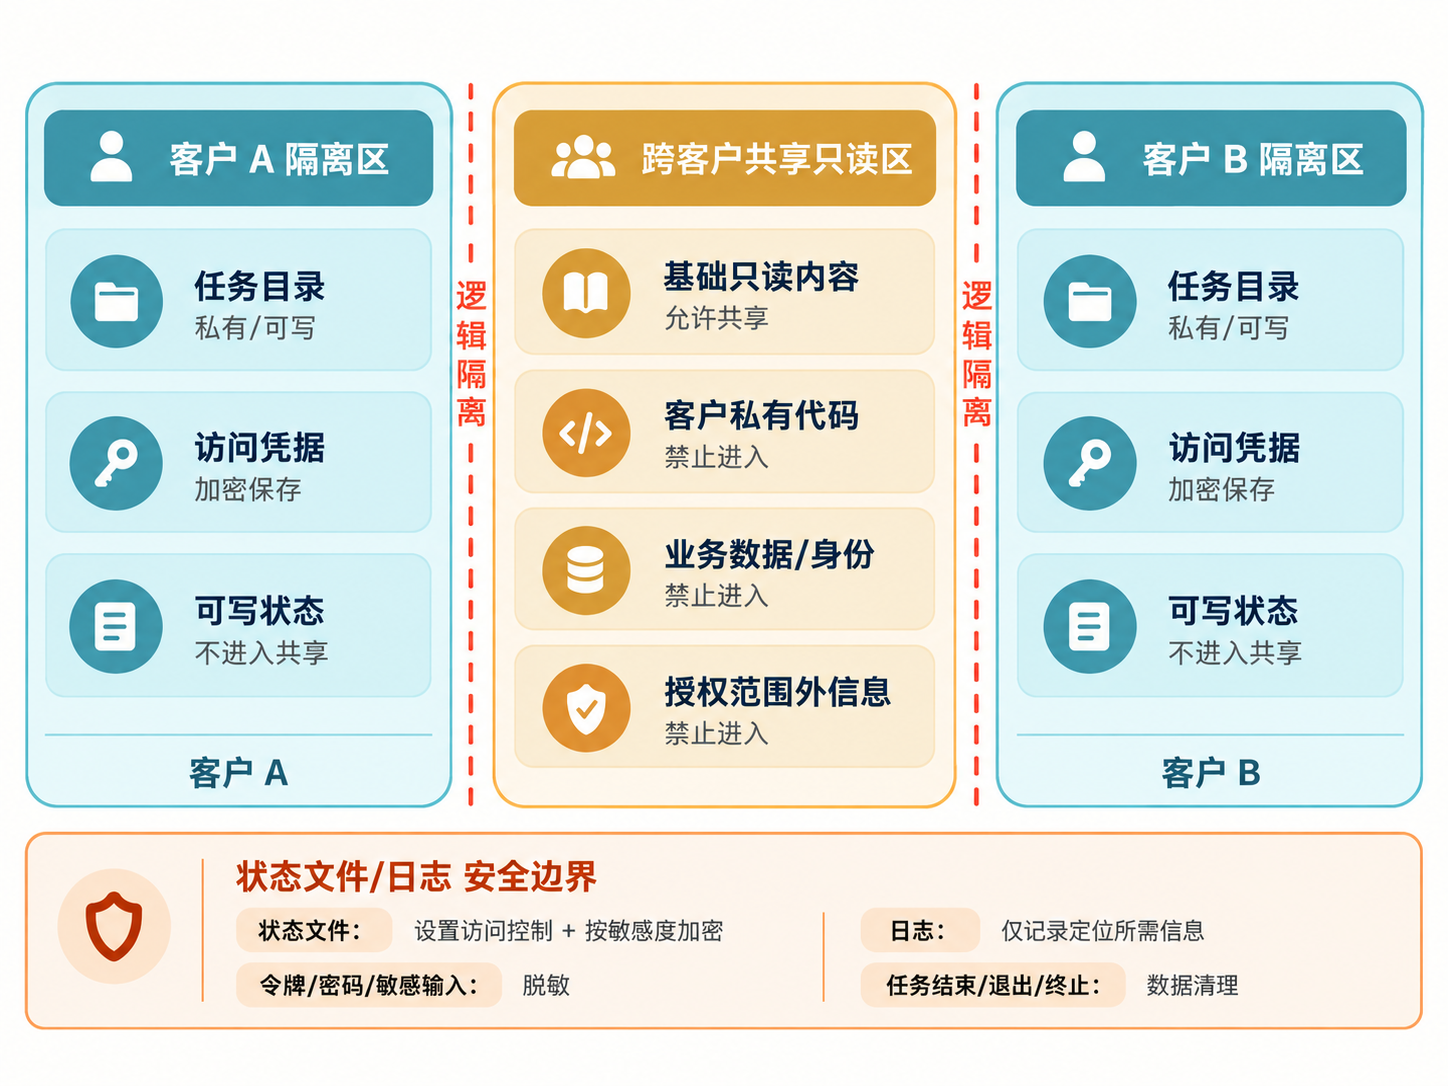
\includegraphics[width=5.1in,keepaspectratio]{figures/image25.png}
\end{center}
\WordFigureCaption{图 7-2 多租户数据与状态隔离边界}

\subsubsection{7.2.6 环境风险}\label{ux73afux5883ux98ceux9669-1}

\NumberedPara{1}{建立分环境验证体系}

优先围绕命题要求的 openEuler、Conch 和 StratoVirt 环境开展适配，分别记录不同处理器架构、系统版本和任务类型的测试结果。

在总内存限制为 16GB、每个沙箱配置为 2U8G、关闭 swap 等条件下，验证指定任务的完成情况和有效并发能力，使测试结果与命题验收直接对应。

\NumberedPara{2}{持续维护兼容性范围}

发布经过验证的软硬件兼容性清单。操作系统、镜像或关键组件升级后，重新检查功能、性能与隔离效果，并为客户保留稳定版本及升级回退路径。

\NumberedPara{3}{根据需求调整商业推进节奏}

结合客户预算和试点结果安排研发优先级。需求不足时控制扩张投入，优先完善能够直接改善客户成本、稳定性和部署效率的功能。

\subsubsection{7.2.7 供应链风险}\label{ux4f9bux5e94ux94feux98ceux9669-1}

\NumberedPara{1}{保证构建和交付可复现}

固定关键代码版本与镜像标识，保存依赖清单、构建脚本和必要的软件包，降低上游更新对已有交付版本的影响。

\NumberedPara{2}{降低单点依赖}

对关键组件和外部服务评估替代方案，将可变接口封装在适配层。替代方案经过验证后再纳入交付范围，逐步提高产品迁移能力。

\NumberedPara{3}{区分外部故障与产品故障}

监控模型接口、存储和网络服务的运行状态，分别记录外部服务失败与沙箱运行失败。针对外部故障设置超时、受控重试和任务暂停机制，减少无效重试造成的资源浪费。

\subsubsection{7.2.8 风险---对策映射汇总表}\label{ux98ceux9669ux5bf9ux7b56ux6620ux5c04ux6c47ux603bux8868}

下表将 7.1 识别的各类风险与 7.2 的对策条目一一对应，并标明责任主体与可量化的监测指标，便于按里程碑检验执行效果。

\begin{longtable}[]{@{}
  >{\centering\arraybackslash}p{(\linewidth - 6\tabcolsep) * \real{0.1018}}
  >{\raggedright\arraybackslash}p{(\linewidth - 6\tabcolsep) * \real{0.4717}}
  >{\centering\arraybackslash}p{(\linewidth - 6\tabcolsep) * \real{0.1171}}
  >{\raggedright\arraybackslash}p{(\linewidth - 6\tabcolsep) * \real{0.3093}}@{}}
\caption*{表 7-2 风险与对策映射表}\tabularnewline
\toprule\noalign{}
\rowcolor{WordTableHeader}
\begin{minipage}[b]{\linewidth}\centering
\TableHeaderText{风险类别}
\end{minipage} & \begin{minipage}[b]{\linewidth}\centering
\TableHeaderText{主要对策（对应条目）}
\end{minipage} & \begin{minipage}[b]{\linewidth}\centering
\TableHeaderText{责任主体}
\end{minipage} & \begin{minipage}[b]{\linewidth}\centering
\TableHeaderText{监测指标 / 验证方式}
\end{minipage} \\
\midrule\noalign{}
\endfirsthead
\toprule\noalign{}
\rowcolor{WordTableHeader}
\begin{minipage}[b]{\linewidth}\centering
\TableHeaderText{风险类别}
\end{minipage} & \begin{minipage}[b]{\linewidth}\centering
\TableHeaderText{主要对策（对应条目）}
\end{minipage} & \begin{minipage}[b]{\linewidth}\centering
\TableHeaderText{责任主体}
\end{minipage} & \begin{minipage}[b]{\linewidth}\centering
\TableHeaderText{监测指标 / 验证方式}
\end{minipage} \\
\midrule\noalign{}
\endhead
\bottomrule\noalign{}
\endlastfoot
\rowcolors{1}{WordTableStripe}{white}
市场风险 & 以真实业务验证采购价值、分阶段推进客户转化、建立可复用的产品与客户结构（7.2.1） & 市场与售前、产品 & 试点客户数及转化率、单一客户收入占比、客户续约与拓展情况、价值报告数据 \\
操作风险 & 建立安全的状态保存与恢复流程）、控制并发恢复和资源峰值、完善发布和交付管理（7.2.2） & 研发、测试 & 任务成功率、恢复正确性、内存占用、关键故障场景测试覆盖、线上故障数 \\
财务风险 & 按阶段安排投入、加强现金流管理、以完整交付成本制定报价（7.2.3） & 财务、经营 & 月度可用资金与应收/预收、各经费科目使用、项目毛利、里程碑达成 \\
法律风险 & 明确成果使用与转化安排、建立开源依赖审查机制、规范合同与对外披露（7.2.4） & 法务、成果转化 & 权属与使用范围清单、许可证合规审查记录、对外披露确认记录 \\
数据与隐私风险 & 限定共享内容和访问范围、加强状态文件与日志保护、建立数据清理与事件响应机制（7.2.5） & 研发、安全、运维 & 访问权限隔离测试、敏感数据脱敏覆盖率、数据清理执行率、疑似泄露事件数及响应时长 \\
环境风险 & 建立分环境验证体系）、持续维护兼容性范围、根据需求调整商业推进节奏（7.2.6） & 研发、测试、产品 & 分环境测试报告、兼容性清单更新频率、版本回退成功率 \\
供应链风险 & 保证构建和交付可复现、降低单点依赖、区分外部故障与产品故障（7.2.7） & 研发、运维 & 依赖清单与构建脚本完备、替代方案验证情况、外部服务故障率与恢复时长 \\
\end{longtable}

\subsection{7.3 风险资本退出}\label{ux98ceux9669ux8d44ux672cux9000ux51fa}

PI OS 将在商业化主体、成果使用权限和经营模式明确后推进融资。以下为拟议的退出安排，具体方式以届时经营状况、投资协议和适用法律为依据。

\subsubsection{7.3.1 项目未达预期目标的退出策略}\label{ux9879ux76eeux672aux8fbeux9884ux671fux76eeux6807ux7684ux9000ux51faux7b56ux7565}

如果项目持续未达到技术交付或商业转化目标，团队将首先分析原因，评估通过缩小产品范围、调整目标客户或转向适配服务能否形成可持续业务。

若调整后仍缺乏可行的经营路径，可与投资者协商股权转让、业务并购或有序终止经营。资产处置仅限商业化主体实际拥有且可依法转让的资产，涉及学校或合作企业的成果，应按照权属和授权约定处理。

退出过程中同步安排客户服务交接、数据迁移与合同履行，以降低对客户及合作方业务连续性的影响。

\subsubsection{7.3.2 设定触发条件的退出策略}\label{ux8bbeux5b9aux89e6ux53d1ux6761ux4ef6ux7684ux9000ux51faux7b56ux7565}

拟在投资协议中明确阶段目标、检查周期和整改期限，将技术交付、客户转化及现金流状况作为持续评估依据。

可协商的触发情形包括：关键验收目标连续未完成、试点长期无法转化为付费业务、可用资金低于约定运营保障线，以及出现影响持续经营的重大安全或权属问题。

触发条件出现后，先启动经营复核和限期整改；整改后仍无法恢复正常推进的，再协商后续融资调整、股权转让或退出安排，避免因单次波动仓促终止项目。

\subsubsection{7.3.3 保护投资者利益的退出策略}\label{ux4fddux62a4ux6295ux8d44ux8005ux5229ux76caux7684ux9000ux51faux7b56ux7565}

项目拟通过定期财务报告、关键经营指标披露、重大支出审议和成果权属核验，提高投资者对资金使用及项目进展的可见度。融资和退出定价以真实经营数据及可核验资产为依据，不承诺保本或固定收益。

股权转让、并购等退出方式，应明确估值依据、付款安排和后续责任。涉及公司清算时，依法清偿相关费用和债务后，股东才参与剩余财产分配；股权投资者不当然优先于债权人受偿。

